\subsection{Data Processing and Mixed Precision Training}
\label{back:data}

\subsubsection{Data Normalization}

Normalization is a technique by which data is transformed from its original scale to a more standard scale \cite{ali2014data}. These techniques are normally used when the dataset has elements of different ranges, and can contribute to faster convergence, and it's why they are as commonly used when preprocessing data. A common method for this is the \textit{minmax} algorithm. This algorithm transforms data to a specified range, most often $[0, 1]$, but it can also be $[-1, 1]$ or any other range. The \textit{minmax} normalization function can be formulated as follows:
\begin{equation}
   x_{\text{normalized}} = \dfrac{x - x_{min}}{x_{max}-x_{min}}
\end{equation}
where $x$ denotes the data, and $x_{min}$ and $x_{max}$ is the minimum and maximum in $x$. 
%
\subsubsection{Half-Precision and Mix-Precision Training}

Working with large datasets and \acrshort{dnn}s can be rather time- and resource-consumptive. One can cast the datatype from single precision to half-precision, along with weights, biases, and losses to address this \cite{micikevicius2018mixed}. This can reduce the loss of accuracy and information, but it lowers memory consumption and decreases training time. \\

\begin{figure}[!h]
    \centering
    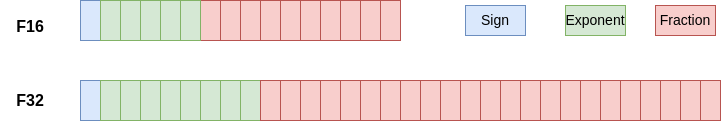
\includegraphics[width=0.8\linewidth]{figures/floats.png}
    \caption{Float16 have a limited amount of bits to represent floating point numbers compared to Float32}
    \label{fig:floats}
\end{figure}
To combat vanishing- or even exploding gradients, we can instead do some operations in \texttt{Float32} while others in \texttt{Float16}. Mixed precision training, introduced in 2018 \cite{micikevicius2018mixed}, is a technique where a neural network's weights, activations, and biases are stored in single precision while the data stays in its original format. It allows for reduced memory consumption while also reducing training times. Additionally, the amount of $\si{\kilo\watt\hour}$ required to train the neural nets would decrease, thus reducing both the cost and the environmental tax of training models. This becomes more important with larger datasets, models, and the sheer amount of \acrshort{gpu}s required to train massive workloads.
%
\subsubsection{Overfitting and Early Stopping}
%
As previously mentioned in Section \ref{back:linear}, overfitting is a common problem within \acrlong{ml}, especially linear layers and dense autoencoders. In addition to popular techniques such as dropout \cite{srivastava2014dropout}, \textit{early stopping} is a regularization technique that aims to avoid overfitting \cite{prechelt2002early}. When training an optimizer such as \acrshort{adam} \cite{kingma2017adam}, or \acrshort{sgd}, one can notice when a model is overfitting by studying the validation loss $L_v$. If $L_v$ starts increasing, the early stop mechanism will stop the training altogether if no improvement of $L_v$ by at least $\epsilon$ is found after $p$ number of epochs. This can described accordingly; we stop at epoch $T$ if:
\begin{equation}
\forall i \in \{T-p+1, ..., T\}: L_v(i) > L_v^* - \epsilon
\end{equation}
where $L_v^*$ is defined as:
\begin{equation}
L_v^* = \min_{j=1}^{T} L_v(j)
\end{equation}
\subsubsection{Parallelism within \acrlong{dl}}
With rapidly evolving deep learning architectures and workloads, the importance of scalable training grows each year. It is estimated that these networks grow $\qty{1.5}{x}$ each year \cite{9499913}, as well as workloads, making parallelization a vital topic in \acrshort{ai} to accommodate ever-increasing memory needs. Several different hardware accelerators have been created to best accommodate these needs; the most apparent of these are \acrshort{gpu}s. By workers, we mainly refer to \acrshort{gpu}s, but this could also be other types of hardware accelerators such as the \acrfull{tpu} \cite{jouppi2023tpu}.
\subsubsection{Data Parallelism}
Data parallelism refers to partitioning data across multiple workers. Given a dataset $X$, we can split $X$ across the workers, store a copy of the model $M$ on each worker, calculate gradients across them all, and update the trainable parameters for $M$. Figure \ref{fig:dataparallel} displays how data can be distributed across multiple \acrshort{gpu}s.
\begin{figure}[!h]
    \centering
    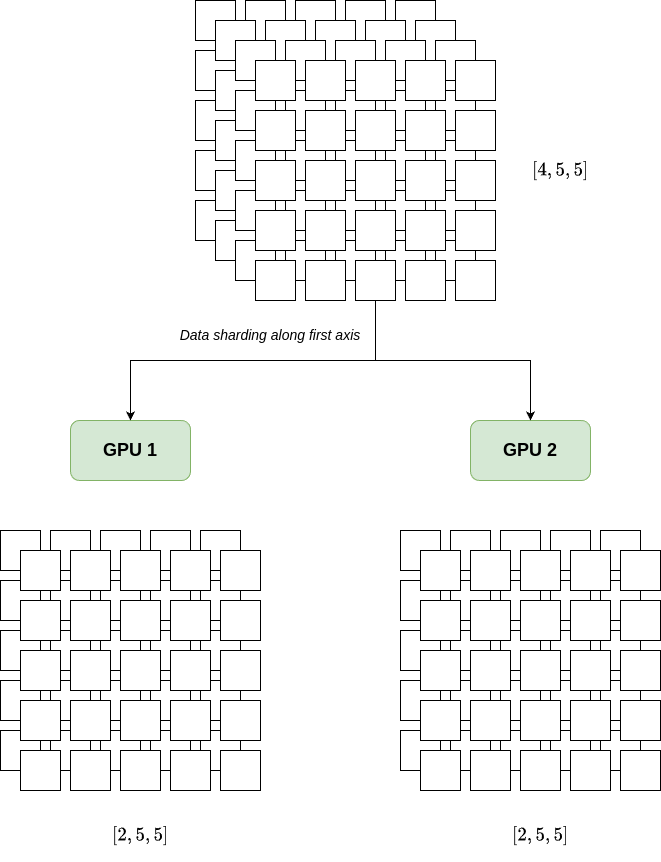
\includegraphics[width=0.6\linewidth]{figures/sharding.png}
    \caption{Example of splitting the workload between to \acrshort{gpu}s. A tensor $M$ of dimensions $[4,5,5]$ is split on the first axis across two \acrshort{gpu}s, leading to each \acrshort{gpu} receiving a tensor of dimension $[2,5,5$].}
    \label{fig:dataparallel}
\end{figure}

